\section{Introduction} \label{introduction}
%% General Introduction
Machine learning techniques are increasingly being used in industrial and scientific applications to gain insight from the data.
Typically, a machine learning pipeline is a series of complex data processing steps to process a labeled training dataset and results in a machine learning model.
The machine learning pipeline is then used to make predictions on new unlabeled data.
To fully utilize the pipeline, it has to be deployed into an environment where it can answer prediction queries in real-time.

%% Intro to the problem of continuous improvement
After the pipeline is deployed, new training data may become available.
In order to adapt to the new training data, one has to train and redeploy the pipeline.
In many real-world use cases, training datasets are very large which may require hours of training to result in a pipeline.
Therefore, it is not feasible to train new pipelines frequently.
This means that the deployed pipeline is not always up-to-date.
Online learning methods are utilized to provide fresh and up-to-date pipelines.
However, unless the online learning method is highly tuned to the specific use case, they do not guarantee a high prediction accuracy \cite{ma2009identifying, macmahan2013}. 
This results in a trade-off between the training cost and accuracy.

%% Use case
\begin{figure}[h!]
\centering
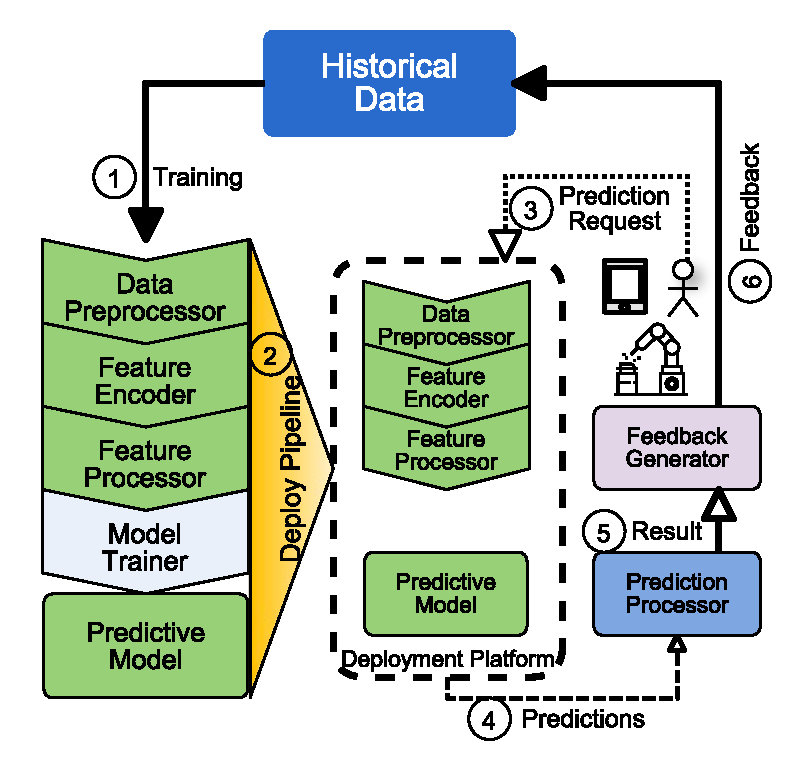
\includegraphics[width=\columnwidth]{../images/generic-motivational-example.pdf}
\caption{Deployment process of machine learning pipelines}
\label{fig:motivational-example}
\end{figure}

Figure \ref{fig:motivational-example} shows the typical lifecycle of a machine learning application in real-world use cases.
From an existing dataset, a pipeline consists of several data and feature processing steps, and training algorithm is trained \textcircled{1}.
Then, a deployment platform deploys this pipeline \textcircled{2} where the pipeline will answer prediction queries arriving at the platform in real-time \textcircled{3}.
The pipeline first processes each prediction request (using the same set of steps used in the training phase) and makes a prediction \textcircled{4}.
The resulting predictions are further processed and converted to meaningful actions before being presented back to the users or the entities issuing the prediction queries  \textcircled{5}.
Based on the result of the prediction query, feedback, containing the original prediction query and the correct label, may be generated that is appended to the existing training data \textcircled{6}.
Throughout the deployment process, it is possible that the accuracy of the predictions being made drop below an acceptable threshold due to changes in the distribution of the incoming prediction requests.
As a result, pipelines are regularly retrained and redeployed back into the deployment platform.

Several real-world use cases follow the workflow described in Figure \ref{fig:motivational-example}.
One example is the problem of Ad click prediction \cite{macmahan2013}.
In Ad click prediction, the pipeline typically consists of extracting features from the users and ads. 
Logistic regression models have shown to perform well in this setting \cite{macmahan2013}.
Prediction queries consist of the user's info and a pool of available ads for displaying to the user.
Once a prediction score for each of these ads are made, an Ads selector unit (similar to the Prediction Processor in the Figure) picks a set of ads with the highest score to display to the user.
Based on the action of the user (click or no click), new training data, containing the original prediction request and the label (+1 for a clicked ad and -1 for a non-clicked ads) will be generated which is stored with the existing training data (similar to the Feedback Generator in the Figure).
\hl{maybe another use case (IoT or Steel coil flatness prediction)}

%% Current Deployment Systems
Many existing platforms, such as Velox \cite{crankshaw2014missing}, Clipper \cite{crankshaw2016clipper}, Laser \cite{agarwal2014laser}, and TensorFlow Extended \cite{baylor2017tfx}, provide support for deployment of machine learning pipelines. 
Since the online training of the models and pipelines may not be adequate to ensure accurate predictions, these platforms, either automatically or manually, facilitate the training and re-deployment of the pipelines and models \cite{crankshaw2014missing}.
In many cases, the amount of training data is very large, thus training a new pipeline may take hours (or even days) \cite{baylor2017tfx}.
During the pipeline training, incoming prediction requests are answered by the old pipeline and new real-time training are accumulated.
By the time the pipeline training data is over, enough data has been accumulated to prompt for a new round of pipeline training.
As a result, in the current deployment platforms, the deployed pipelines are out of date which results in lower prediction accuracy.

%% Our solution
We propose a deployment platform that continuously updates the pipelines (thus providing up-to-date pipelines) using a combination of the historical and incoming data.
Our deployment platform updates the pipeline using the incoming feedback data (we call this the real-time training data) similar to how online machine learning algorithms work and performs small batch updates using the historical data.
Our solution offers two key optimizations.

\textit{Proactive training.}
Instead of fully training a new pipeline using the historical training data, we continuously update the existing pipeline using small sampled batches of the historical data.
The deployment platform forwards each batch of the data through the pipeline and performs a partial model update using this batch.
The updated pipeline is immediately ready for answering prediction queries.
Our experiments show that proactive training of the pipeline achieves more accurate predictions over time and requires fewer resources when compared to the full pipeline retraining.

\textit{Online Statistics Computation and Data Materialization}
Our deployment platform updates the pipeline using the real-time training data by employing advanced online machine learning algorithms (such as Adagrad \cite{duchi2011adaptive}), before storing it for the proactive training.
Since the real-time training data is traveling through the pipeline during the online training phase, we compute statistics required by the pipeline, update the pipeline components, and transform and materialize the data before storing it with the rest of the historical data.
As a result, during the proactive training, the data processing and the feature processing steps of the pipeline are skipped and the materialized data is directly used in the model trainer component of the pipeline.

% Our contributions
In summary, our contributions are:
\begin{itemize}
\item A platform for continuously training deployed machine learning pipelines that adapts to the rate of the incoming data.
\item Proactive training of the deployed pipelines that frequently updates the pipeline in-place using a combination of the historical and the real-time data and increases the prediction accuracy when compared with state of the art.
\item Efficient pipeline training by online statistics computation and data materialization, thus guaranteeing the availability of up-to-date pipelines for answering prediction queries.
\end{itemize}

The rest of this paper is organized as follows:
Section \ref{continuous-training-serving} describes the details of our continuous training approach.
In Section \ref{sec:system-architecture}, we introduce the architecture of our deployment system.
In Section \ref{evaluation}, we evaluate the performance of our continuous deployment approach.
Section \ref {related-work} discusses the related work.
Finally, Section \ref{conclusion} presents our conclusion and the future work.
